\section{Ejercicio \#1: Comparación de Monedas}

\subsection{Problema a resolver}

Se tiene una bolsa con $n$ monedas de igual denominación, de las cuales exactamente una es falsa y es más liviana que el resto.
El objetivo es identificar la moneda falsa sin ordenar por peso y haciendo uso de División y Conquista.

\subsection{Algoritmo de División y Conquista}

La entrada del algoritmo es una lista de monedas representadas por su peso. Se asume que todos los pesos son iguales, a
excepción del peso de la moneda falsa, es decir: $[b, b, a, b, b]$ donde $a < b$.

En cada paso el algoritmo parte la lista en dos mitades y calcula el \textbf{promedio} de cada parte. Usar el promedio
en lugar de la suma garantiza correctitud cuando $n$ es impar, ya que ambas mitades pueden tener tamaños distintos.

\begin{enumerate}
	\item Si el promedio izquierdo es menor al promedio derecho, la moneda falsa está en la mitad izquierda: se recursa sobre ella.
	\item Si el promedio derecho es menor al promedio izquierdo, la moneda falsa está en la mitad derecha: se recursa sobre ella.
\end{enumerate}

Casos base:

\begin{enumerate}
	\item Si la lista tiene longitud uno, se retorna ese único elemento como la moneda falsa.
	\item Si la lista tiene longitud dos, se retorna la moneda de menor peso entre los dos elementos.
\end{enumerate}

\textbf{Pesadas en el algoritmo:}

Las pesadas son la cantidad de veces que se usa la balanza para comparar grupos de monedas. En el algoritmo se registra
una pesada cada vez que se calculan y comparan los promedios de ambas mitades, y también en los casos base (listas de
longitud uno o dos).

\textbf{Estructuras de datos:} El algoritmo opera sobre una lista de
enteros que representan los pesos de las monedas. Los parámetros
\texttt{inicio} y \texttt{fin} son índices enteros que delimitan el
subarreglo activo en cada llamada recursiva, evitando copias. El
\texttt{contador} se pasa por referencia (lista de un elemento) para
acumular la cantidad de pesadas a través de las llamadas recursivas.

\textbf{Solución:}

\lstinputlisting[]{code/monedas.txt}

\subsection{Seguimiento del algoritmo}

Tomamos como ejemplo $n = 8$ monedas: $[10, 10, 10, 10, 4, 10, 10, 10]$
donde la moneda falsa (peso 4) está en la posición 4.

\begin{table}[h]
\centering
\begin{tabular}{c c c c c c}
\hline
Paso & inicio & fin & $\overline{x}_{izq}$ & $\overline{x}_{der}$ & Decisión \\
\hline
1 & 0 & 7 & $\frac{40}{4}=10$ & $\frac{34}{4}=8.5$ & Recursar derecha \\
2 & 4 & 7 & $\frac{14}{2}=7$   & $\frac{20}{2}=10$  & Recursar izquierda \\
3 & 4 & 5 & $4$               & $10$               & Caso base: retorna 4 \\
\hline
\end{tabular}
\caption{Seguimiento del algoritmo para $n=8$, falsa en posición 4.}
\label{tab:ej1-seguimiento}
\end{table}

En 3 pesadas se identificó la moneda falsa, consistente con
$\lceil \log_2 8 \rceil = 3$.

\subsection{Complejidad temporal y cantidad de pesadas}

El algoritmo es de Divide y Conquista con la siguiente estructura en cada llamada:
\begin{itemize}
	\item Se divide la lista en dos mitades: $O(1)$.
	\item Se calcula el promedio de cada mitad con \texttt{sum()}: $O(n)$ en total.
	\item Se recursa sobre \textbf{una sola} mitad.
\end{itemize}

La ecuación de recurrencia resultante es:

\[
T(n) = T\!\left(\frac{n}{2}\right) + O(n)
\]

donde $A = 1$ (una sola llamada recursiva), $B = 2$ (el problema se divide a la mitad), y el costo adicional en cada nivel es $O(n)$ por el cálculo de \texttt{sum()} sobre ambas mitades.

Aplicando el \textbf{Teorema Maestro} en la forma simplificada, la ecuación de recurrencia general se define como:
\[
\mathcal{T}(n) = A\mathcal{T}\left(\frac{n}{B}\right) + \mathcal{O}(n^C)
\]
De acuerdo con este teorema, la resolución de la complejidad se divide en tres casos según la relación comparativa entre $\log_B(A)$ y $C$:
\begin{itemize}
    \item \textbf{Si } $\log_B(A) < C \longrightarrow \mathcal{T}(n) = \mathcal{O}(n^C)$
    \item \textbf{Si } $\log_B(A) = C \longrightarrow \mathcal{T}(n) = \mathcal{O}(n^C \log_B n) = \mathcal{O}(n^C \log n)$
    \item \textbf{Si } $\log_B(A) > C \longrightarrow \mathcal{T}(n) = \mathcal{O}(n^{\log_B A})$
\end{itemize}

Para nuestra ecuación de recurrencia particular, $T(n) = T\left(\frac{n}{2}\right) + \mathcal{O}(n)$, los valores de los parámetros obtenidos son:
\begin{itemize}
    \item $A = 1$
    \item $B = 2$
    \item $C = 1$ \quad (ya que $\mathcal{O}(n) = \mathcal{O}(n^1)$)
\end{itemize}

Procedemos a evaluar el logaritmo base $B$ de $A$:
\[
\log_B(A) = \log_2(1) = 0
\]

Al comparar el resultado con el exponente $C$, se verifica que $0 < 1$ ($\log_B(A) < C$), lo que nos posiciona estrictamente en el \textbf{primer caso} del teorema. Por lo tanto, la complejidad temporal final del algoritmo está determinada por dicho caso:
\[
\mathcal{T}(n) = \mathcal{O}(n^C) \implies \boxed{T(n) = \mathcal{O}(n)}
\]

\textbf{Cantidad de pesadas:}

Dado que el algoritmo recursa sobre una sola rama en cada nivel, la profundidad del árbol de recursión es
$\lceil \log_2 n \rceil$, y se realiza exactamente una pesada por nivel. La cantidad de pesadas sigue:

\[
\text{Pesadas}(n) = O(\log_2 n)
\]

A diferencia de algoritmos como Merge Sort, este algoritmo \textbf{no
requiere un paso de combinación}: una vez que se recursa sobre la mitad
que contiene la moneda falsa, el resultado se retorna directamente sin
necesidad de combinar resultados de ambas ramas.

\subsection{Metodología adoptada}

Se evaluó el algoritmo con sets de datos de distintos tamaños:
\[
n \in \{100,\ 500,\ 1000,\ 5000,\ 10000,\ 50000,\ 100000,\ 200000,\ 500000,\ 1000000\}
\]
Para cada tamaño se generó un archivo con $n$ monedas genuinas de peso 10 y una única moneda falsa de peso 4 en una
posición aleatoria. Los tiempos reportados se obtuvieron ejecutando el script de benchmarking:

\begin{verbatim}
python ejercicios/ej-dyc/run_all_inputs.py
\end{verbatim}

El script importa directamente la función \texttt{encontrar\_moneda\_falsa}, realiza una ejecución de \textit{warm-up}
para descartar efectos de caché fríos, y luego mide 20 repeticiones con \texttt{time.perf\_counter()}, reportando el
tiempo promedio en microsegundos junto con la cantidad de pesadas.

\subsection{Resultados y gráficos}

\begin{table}[h]
    \centering
    \begin{tabular}{r r r}
    \hline
    $n$ & Tiempo (s) & Pesadas \\
    \hline
    100 & 0.000057 & 7 \\
    500 & 0.000096 & 10 \\
    1000 & 0.000076 & 11 \\
    5000 & 0.000214 & 13 \\
    10000 & 0.000358 & 15 \\
    50000 & 0.001458 & 17 \\
    \hline
    \end{tabular}
    \caption{Resultados experimentales del ejercicio 1.}
    \label{tab:ej1-resultados}
\end{table}


\begin{figure}[H]
	\centering
	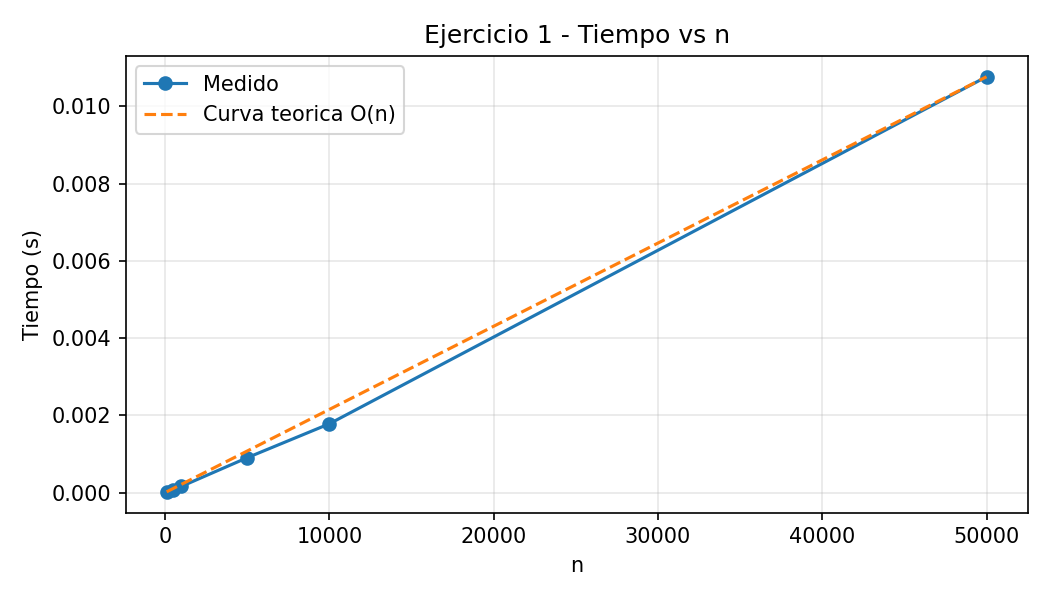
\includegraphics[width=0.85\textwidth]{img/ej1_tiempos.png}
	\caption{Tiempo de ejecución en escala log-log con curvas de referencia $O(\log n)$, $O(n)$, $O(n \log n)$ y $O(n^2)$.
	         Los datos siguen la recta de pendiente~1, confirmando $T(n) = O(n)$.}
	\label{fig:ej1-tiempos}
\end{figure}

\begin{figure}[H]
	\centering
	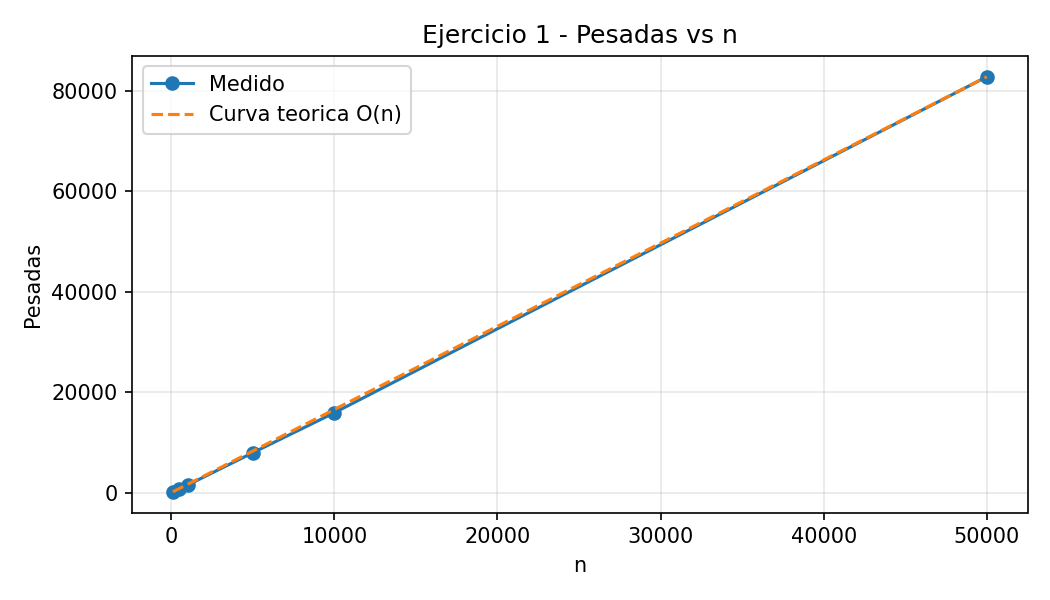
\includegraphics[width=0.85\textwidth]{img/ej1_pesadas.png}
	\caption{Cantidad de pesadas vs tamaño del array en escala semi-log.
	         Los puntos se alinean sobre la curva $c \cdot \log_2 n$, confirmando $\text{Pesadas}(n) = O(\log_2 n)$.}
	\label{fig:ej1-pesadas}
\end{figure}

Los gráficos confirman el análisis teórico: el tiempo de ejecución crece linealmente con $n$, mientras que la cantidad
de pesadas crece logarítmicamente.

\subsection{Relación entre tiempo de ejecución y pesadas}

El tiempo de ejecución y la cantidad de pesadas tienen \textbf{complejidades distintas}:

\begin{itemize}
	\item \textbf{Tiempo:} $O(n)$, dominado por el cómputo de \texttt{sum()} en cada nivel de recursión. Aunque solo se
	      recursa una rama, el cálculo de los promedios recorre ~$n/2$ elementos en el primer nivel, $n/4$ en el
	      segundo, etc., sumando en total $\approx 2n$ operaciones.
	\item \textbf{Pesadas:} $O(\log_2 n)$, ya que se realiza exactamente una comparación de grupos por nivel, y el
	      árbol tiene profundidad $\lceil \log_2 n \rceil$.
\end{itemize}

La distinción es relevante según qué se considere la \textit{operación elemental}: si se modela el problema con una
balanza de platillos donde pesar un grupo completo cuenta como una sola operación, el costo relevante es $O(\log n)$
pesadas. Si se considera el costo computacional real (calcular la suma), el costo es $O(n)$.

\subsection{Posible optimización: evitar el recálculo de sumas}

Una optimización natural consiste en propagar la suma del segmento activo como parámetro de la llamada recursiva.
En cada nivel, en lugar de calcular \texttt{sum()} sobre ambas mitades, se calcula la suma de \textbf{una sola mitad}
en $O(n/2)$ y la suma de la otra se obtiene por resta en $O(1)$:

\[
\text{suma\_der} = \text{suma\_total} - \text{suma\_izq}
\]

La recurrencia resultante es:

\[
T(n) = T\!\left(\frac{n}{2}\right) + O\!\left(\frac{n}{2}\right) = T\!\left(\frac{n}{2}\right) + O(n)
\]

dado que $O(n/2) = O(n)$, el Teorema Maestro sigue aplicando con los mismos parámetros y la complejidad asintótica
\textbf{no cambia}: $T(n) = O(n)$.

Sin embargo, la constante oculta se reduce a la mitad. En el algoritmo original el trabajo acumulado por nivel es:
\[
n + \frac{n}{2} + \frac{n}{4} + \cdots \approx 2n \text{ operaciones}
\]
Con la optimización, al calcular solo una mitad por nivel:
\[
\frac{n}{2} + \frac{n}{4} + \frac{n}{8} + \cdots \approx n \text{ operaciones}
\]
Es decir, se obtiene una mejora práctica de $\approx 2\times$ en velocidad sin modificar la clase de complejidad.

\subsection{Conclusión}

El algoritmo de División y Conquista para identificar la moneda falsa
presenta dos métricas de complejidad distintas según la operación que se
considere elemental:

\begin{itemize}
    \item \textbf{Tiempo de CPU:} $O(n)$, ya que en cada nivel de recursión
    se computan las sumas de ambas mitades del arreglo, acumulando un total
    de aproximadamente $2n$ operaciones aritméticas.
    \item \textbf{Pesadas de balanza:} $O(\log_2 n)$, ya que el algoritmo
    realiza exactamente una comparación de grupos por nivel y el árbol de
    recursión tiene profundidad $\lceil \log_2 n \rceil$.
\end{itemize}

Los resultados experimentales confirman ambas predicciones: en el gráfico
log-log, los tiempos siguen la recta de pendiente 1 correspondiente a
$O(n)$, mientras que en el gráfico semi-log, la cantidad de pesadas se
alinea sobre la curva $c \cdot \log_2 n$.

La distinción entre ambas complejidades es relevante en el contexto del
problema: si se modela con una balanza de platillos donde pesar un grupo
completo cuenta como una sola operación, el costo práctico es
$O(\log_2 n)$ pesadas — óptimo para este tipo de problema.
